\documentclass[11pt, letterpaper]{article} % El tamaño de letra se cambia acá (podrían poner [10pt], por ejemplo)

\usepackage[main=spanish, english]{babel}
\usepackage[utf8x]{inputenc}
\usepackage{fullpage}
\usepackage{euscript}
\usepackage{amsmath}
\usepackage{amssymb}
\usepackage[amssymb]{SIunits}
\usepackage[pdftex]{graphicx}
\usepackage[colorlinks=false, linkcolor=blue, urlcolor=blue, pdfborder={0 0 0}]{hyperref}
\usepackage{graphics}
\usepackage{subcaption}
\usepackage{eurosym} 
\usepackage[version=3]{mhchem} 
\usepackage{enumerate}
\usepackage{epsfig}
\usepackage{float}
\usepackage{tikz}
\usetikzlibrary{babel,arrows,automata}
\usepackage{listings} 
\usepackage[americanvoltages]{circuitikz}
%paquetes para utilizar normas apa
\usepackage{apacite}
\usepackage{tabularx}


\RequirePackage{apacite}

% Título del documento. Cámbienlo dependiendo del propósito del documento
\title{Escuela de Ciencias Físicas y Matemáticas}
\makeatletter
\let\thetitle\@title
\makeatother

%Acá definen características del encabezado. Pueden jugar cambiando números y viendo el efecto sobre el encabezado.
\newcommand{\hoofding}[5]{ %El [5] quiere decir que se escribirán 5 ítems
\begin{flushleft}

\includegraphics[height=2.8cm]{images/logoecfm.png} %[height=] define el tamaño (altura en este caso) de la imagen [Logo.jpeg]
\end{flushleft}
\vspace{-3cm} % Relacionado con la distancia entre el logo y la línea
\hspace{4cm} 
\parbox{15cm}{ #1\\#2\\#3\\#4\\#5} % Cada # indica en qué ítem irá qué información
{\parindent=0pt \hrulefill} 
\vspace{1mm}}

% Invocar figura
%\newcommand{\figuur}[2]{\includegraphics[width=#1]{#2}} 
%\setlength{\parindent}{0pt}
%\setlength{\parskip}{1ex plus 0.5ex minus 0.2ex}

% Aquí inician su documento
\begin{document}
\setlength{\parindent}{1cm}%sangría
%\renewcommand{\BOthers}[1]{et al.\hbox{}}%esto cambia para multiples autores de "Cols" a "et al." respetando lo propuesto por normas apa.
%\renewcommand{\BRetrievedFrom}{Recuperado de }%esto cambia la palabra "Descargado de" a "Recuperado de" respetando lo propuesto por normas apa.

% En esta parte indican los ítems del encabezado (por ejemplo #1 era Curso, #2 era código... y así)
\hoofding {\thetitle}{Laboratorio de Electrónica Digital (F604)}{Practica $\#$2}
{\textit{HMI con lógica combinacional}}{Ing. Iván René Morales}%se substituye por sus nombres

% Acá incluyen el cuerpo de su documento, que está en el archivo Cuerpo.tex
% Para iniciar una sección debe escribirse
%\section{Nombre de la sección}
% Lo anterior inmediatamente creará la sección y la numerará.

\section*{Objetivos}
\subsection*{Generales}
\begin{itemize}
    \item Realizar una interfaz básica humano-máquina (HMI) con un circuito digital utilizando dispositivos de entrada y salida simples
\end{itemize}

\subsection*{Específicos}
\begin{itemize}
    \item Diseñar múltiples circuitos combinacionales para obtener un resultado único en conjunto
    \item Implementar un circuito de lógica combinacional utilizando compuertas lógicas básicas y un circuito de propósito específico para la decodificación de BCD a formato de Display de 7 segmentos
    \item Contrastar los diseños teóricos con los resultados experimentales de los circuitos implementados físicamente
\end{itemize}

\section{Introducción}

\subsection{Interfaz humano-máquina (HMI)}
Es un método de interacción entre un dispositivo (normalmente computadora o maquinaria) y un humano. Este proceso de interacción debe ser lo más natural que sea posible para el humano, 
tanto para enviar comandos, como para recibir retroalimentación de parte de la máquina con la que se trabaja. Las interfaces se realizan a través de dispositivos de entrada y dispositivos de salida.

En esta práctica los elementos de entrada son lo más los pulsadores o el \emph{dip-switch} y los elementos de salida de la interfaz son los LEDs y el display de 7 segmentos.
Estos elementos son los más básicos que pueden utilizarse en un circuito digital para interactuar naturalmente un usuario humano sin necesidad de un entrenamiento especial.

\subsection{Display de 7 segmentos}
La probabilidad de que un usuario promedio sea capaz de decodificar en tiempo real la información desplegada en 4 LEDs en BCD 
es demasiado baja (incluso peor es medir voltajes o estados lógicos en 4 salidas al mismo tiempo).
Por esta razón incluso ya en la década de 1970 las calculadoras científicas incluían una forma más amigable de mostrar
la información a sus usuarios. Un dato curioso es que en los 70's y 80's la tecnología electrónica de cómputo era exactamente la misma
que se basan ustedes en este laboratorio y aún así los dispositivos eran bastante complejos (por ejemplo las calculadoras de \emph{Hewlett-Packard} HP-35, HP-41cx y HP-42s).

¡Imagine al módulo lunar del Apollo 11 mostrando información codificada en BCD a los astronautas para las instrucciones de alunizaje y escape de órbita!
Hubiese sido una tarea (más) titánica comandar el vehículo si la retroalimentación fuese en el lenguaje que solo la computadora de a bordo entendiese (y no los humanos que la comandaban).

\vspace{14pt}

El display de 7 segmentos es un dispositivo de interfaz de salida genérico capaz de desplegar caracteres hexadecimales (0, 1, 2, 3, 4, 5, 6, 7, 8, 9, A, B, C , D , E, F) utilizando solamente
7 LEDs dispuestos en forma de barra (Figura \ref{Fig:SevenSegment}).

\begin{figure}[H]
    \centering
    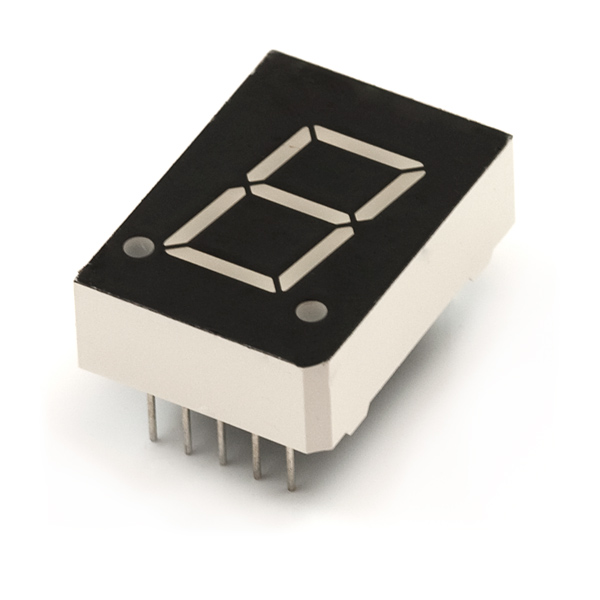
\includegraphics[scale=0.3]{images/7SegmentDisplay.jpg}
    \caption{Display de 7 segmentos}
    \label{Fig:SevenSegment}
\end{figure}

Cada LED (barra) del display se controla individualmente y tiene asignado un código único. Normalmente la asignación de los segmentos
depende de la posición y se enumeran desde \emph{A} hasta \emph{G}. Incluso, algunos display contienen también un punto decimal (llamado \emph{DP}).
En la Figura \ref{Fig:SevenSegments} se muestra la nomenclatura correspondiente a cada segmento del display.


\begin{figure}[H]
    \centering
    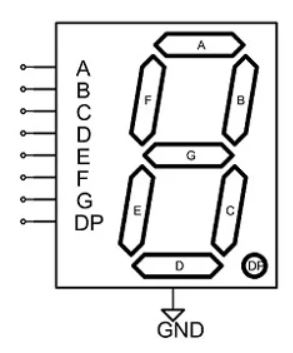
\includegraphics[scale=0.8]{images/DisplaySegments.JPG}
    \caption{Compuertas dentro de un Circuito Integrado}
    \label{Fig:SevenSegments}
\end{figure}

Para desplegar un caracter específico, se activan segmentos (LEDs) específicos en el display.

En la Figura \ref{Fig:DisplayCharacters} se muestran algunos ejemplos:

\begin{itemize}
    \item \textbf{Caracter 5}: Segmentos A, C, D, F, G
    \item \textbf{Caracter 7}: Segmentos A, B, C
    \item \textbf{Caracter 8}: Segmentos A, B, C, D, E, F, G
\end{itemize}

\begin{figure}[H]
    \centering
    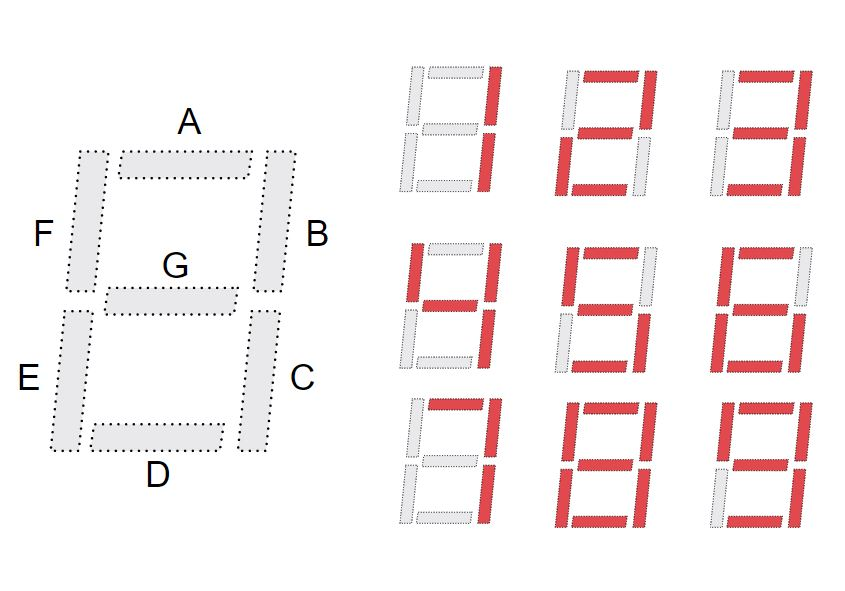
\includegraphics[scale=0.5]{images/DisplayCharacters.JPG}
    \caption{Compuertas dentro de un Circuito Integrado}
    \label{Fig:DisplayCharacters}
\end{figure}

\subsubsection{Métodos de activación de display}
El elemento funcional básico del display es un LED en disposición de barra. Los 7 (u 8) LEDs están expuestos al diseñador del circuito a través
de los pines del empaquetado. Cada LED posee un ánodo y un cátodo (positivo y negativo), por lo que en teoría eso significa 14 pines en total (asumiendo
que no existe LED para mostrar un punto decimal). Sin embargo, dado que el mecanismo de funcionamiento del display consiste nada más en activar y desactivar
LEDs individuales, la forma más simple de hacer esto es polarizar adecuadamente cada diodo y que exista corriente a través de él. Por lo tanto,
el display de 7 segmentos está diseñado de tal forma que todos los ánodos (terminales positivas) de los 7 LEDs que lo conforman
estén interconectados entre sí (y se alimentan directamente de los 5V), mientras cada cátodo (terminal negativa) se activa
individualmente completando el circuito a tierra (GND) a través de una resistencia limitadora de corriente. A este tipo de display de 7 segmentos se le
conoce como \emph{Display de Ánodo Común}. A continuación una descripción de cada tipo de display.

\begin{itemize}
    \item \textbf{Ánodo común}: Los \underline{ánodos} de los LEDs se encuentran conectados internamente y deben llevarse directamente a 5V y los cátodos se activan colocando un potencial 0V (GND). En otras palabras,
    el funcionamiento es lógica negada (se activa con un 0 y se desactiva con un 1 lógico).
    \item \textbf{Cátodo común}: Los \underline{cátodos} de los 7 LEDs están interconectados. Éste único pin se conecta a 0V (GND) y los ánodos se activan individualmente colocando un 
    nivel alto (1 lógico). En resumen: se activa con 1 y se desactiva con 0.
\end{itemize}

En esta práctica se utilizará un display de \textbf{ánodo común}, ya que es el comercialmente disponible en la mayoría de tiendas de electrónica.
En la Figura \ref{Fig:CommonAnode} se muestra el funcionamiento interno de un display de este tipo.

\begin{figure}[H]
    \centering
    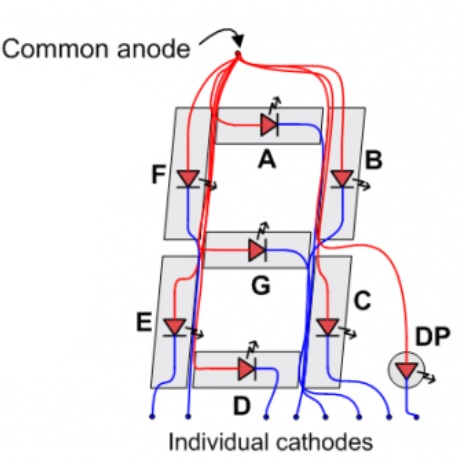
\includegraphics[scale=0.5]{images/CommonAnode.jpg}
    \caption{Display de 7 segmentos de ánodo común}
    \label{Fig:CommonAnode}
\end{figure}

\subsection{Representación numérica de bases distintas de 10}
A pesar de ser un tema que comúnmente se abarca en los cursos básicos de programación, es importante recordar que para representar valores
en una base numérica distinta a la decimal existen estándares que permiten la interoperabilidad entre los sistemas. A continuación algunos ejemplos
de representación en distintas bases (el \textbf{*} indica cualquier símbolo válido de la base):

\begin{itemize}
    \item Binario     - 0b**** (ejemplo: 0b1101)
    \item Octal       - 0***** (ejemplo: 041472)
    \item Hexadecimal - 0x**** (ejemplo: 0x30FA)
\end{itemize}

\subsection{Decodificador BCD a 7 segmentos - 74LS47}
Este circuito integrado de uso específico cumple con una tarea única: obtener de una entrada codificada en BCD de 4 bits
(valores entre 0x00 y 0x0F) y convertirlos a la representación de segmentos (A - G) de un display de 7 segmentos. Específicamente
el modelo 74LS47 está diseñado para manejar displays de ánodo común. Este integrado también incluye algunos pines extra de entrada para
realizar pruebas de funcionamiento del display (\emph{LAMP TEST}, \emph{BI/RB0}, \emph{RBI}), los cuales no serán utilizados en esta práctica. En la Figura \ref{Fig:74LS47} se muestra
un diagrama de conexión para este dispositivo. La hoja de datos completa puede descargarse de la siguiente dirección:

\begin{center}
    \url{http://www.sycelectronica.com.ar/semiconductores/74LS47.pdf}    
\end{center}


\begin{figure}[H]
    \centering
    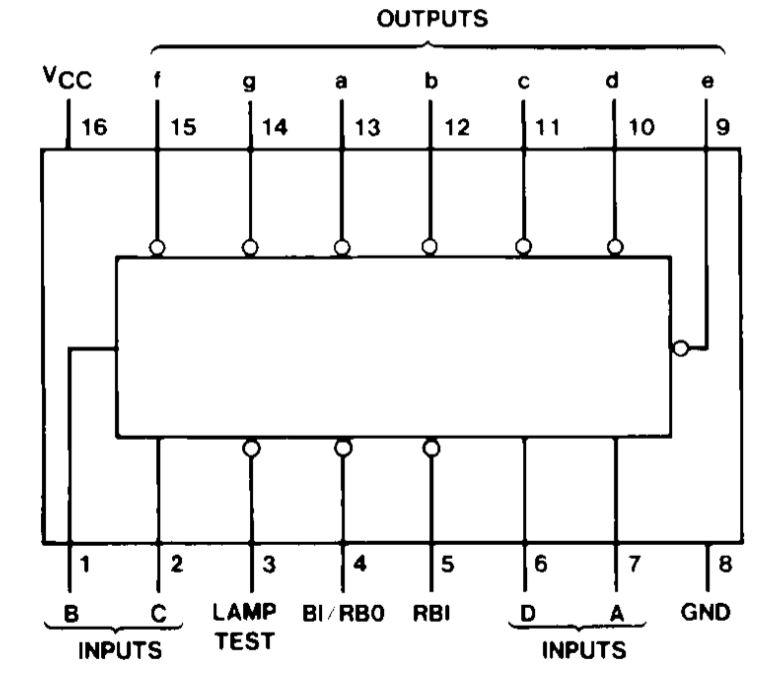
\includegraphics[scale=0.8]{images/74LS47.JPG}
    \caption{Diagrama de conexión de 74LS47}
    \label{Fig:74LS47}
\end{figure}



\pagebreak

\section{Desarrollo Experimental}
\subsection{Materiales y Equipo}

Cada grupo debe llevar su material y equipo de trabajo durante las prácticas. Pregunte a su profesor qué \emph{Equipo de Laboratorio} puede ser prestado
de parte del laboratorio de instrumentación. El laboratorio de instrumentación no tiene disponibilidad de ningún elemento de la lista \emph{Materiales}.

\subsubsection*{Materiales}
\begin{itemize}
    \item 1x dip-switch de 4 posiciones (o más)
    \item 4x pulsadores (si no consiguiesen el dip-switch de 4 posiciones)
    \item 1x fuente de alimentación (ver apartado anterior con todas las alternativas)
    \item 2x capacitores electrolíticos de 47 $\mu$F 16V
    \item 2x capacitores cerámicos de 100nF 25V
    \item 4x resistencias de 10 k$\ohm$
    \item 4x LEDs de cualquier color
    \item 1x Display de 7 segmentos de \textbf{ánodo común} de cualquier color
    \item 7x Resistencias $220 \ohm \leq R \leq 1 k\ohm$
    \item 6x metros de alambre para protoboard calibre 22. Compren al menos 2 colores para los 6 metros. \textbf{No usen \emph{UTP}}, aunque eso les quieran vender.
    \item 1x Circuito Integrado 74LS47 (decodificador BCD a Display 7 segmentos ánodo común)
    \item Las compuertas lógicas a utilizar dependen del diseño final de cada grupo (AND, OR, NOT)
\end{itemize}


\subsubsection*{Equipo de Laboratorio}
\begin{itemize}
    \item 1x Pinzas delgadas
    \item 1x Cortaalambres
    \item 1x Pelador de alambres para calibre 22 (opcional)
    \item 1x Tijeras pequeñas o cortauñas (si no tienen pela alambres)
    \item 1x Protoboard de al menos 2 galletas (puede juntar 2 protoboards de 1 galleta)
    \item 1x Multímetro digital para medir voltaje
\end{itemize}

\subsection{Procedimiento}
\subsubsection{Fuente de alimentación}
Utilice la misma fuente de alimentación que en la Práctica \#1.

\subsubsection{Decodificador de índice / Multiplexor}
Se requiere a diseñar un circuito de lógica digital que permita decodificar la información de año de ingreso a la USAC de alguno de los
integrantes del grupo a un valor que exprese un índice correspondiente a cada dígito. Debido a que la cantidad de dígitos
que conforman este número es 4, se puede realizar la decodificación de entrada BCD utilizando 3 bits.

\vspace{14pt}

Por ejemplo: si el año de ingreso fuese \emph{2018}, se le asignaría un índice (posición) a cada dígito como se
muestra en la Tabla \ref{Table:ejemploIndices}.

\begin{table}[H]
    \centering
    \begin{tabular}{|c|c|c|c|c|}
        \hline
        \textbf{Dígito} & 2 & 0 & 1 & 8 \\ \hline
        \textbf{Índice}  & 1 & 2 & 3 & 4 \\ \hline
    \end{tabular}
    \caption{Ejemplo de asignación de índice a cada dígito}
    \label{Table:ejemploIndices}
\end{table}


En otras palabras, el \textbf{índice 2} corresponde al \textbf{dígito 0}; al \textbf{índice 3} le corresponde el \textbf{dígito 1} y de la misma forma para el resto...

\vspace{14 pt}

El objetivo de esta sección será diseñar y construir un circuito que codifique cada uno de los índices (del 1 al 4) al dígito correspondiente en el año a mostrar.
Las salidas deben ser la representación en BCD de cada dígito, asignado al índice de cada entrada.

\vspace{14 pt}

El método de entrada es a través del dip-switch (no olivde las resistencias \emph{pull-down}) de 3 posiciones, en el que el usuairo
selecciona un valor de índice (de 1 a 4) y la salida es el dígito correspondiente al índice,
la cuál se despliega a través de 4 LEDs (siempre con sus resistencias limitadoras de corriente).

\subsubsection*{Importante}
\begin{itemize}
    \item Si el usuario selecciona un índice inválido (0, 5, 6, 7) la salida del circuito debe ser siempre $1111_2$
    \item Tome en cuenta que la salida debe ser de 4 bits, ya que un dígito puede tener un valor entre 0 y 9.
    \item Cada grupo de trabajo puede seleccionar un número a decodificar, no necesariamente puede ser un año. El único requisito es que tenga al menos 4 dígitos.
\end{itemize}

\subsection{Interfaz de salida}
En esta sección convertirán la información BCD en un número humanamente amigable: el display de 7 segmentos es la forma más sencilla de lograr
el elemento de salida de la interfaz humano-máquina. Se utilizará un circuito integrado decodificación de BCD a Display para esta tarea.

Por primera vez se le dejará como tarea interpretar una hoja de datos de fabricante, en este caso, para comprender el funcionamiento detallado y
conexionado del 74LS47. Cualquier duda consúltela a su instructor. Consejo: no se enfoque en el diagrama lógico que aparece en la hoja de datos,
utilice mejor la tabla de verdad y las descripciones de cada pin. Las primeras 2 páginas de la hoja de datos contienen toda la información necesaria
para realizar la práctica.

\subsubsection*{Importante}
Recuerde que al trabajar con un display de ánodo común, la activación de un elemento se hace através de un \textbf{0 lógico}. No olvide esto
al estar analizando la tabla de verdad en la hoja de datos del integrado.

\subsubsection{Resistencias de cátodos}
Para limitar la corriente que circula en cada uno de los LED que conforman el display es necesario colocar una resistencia individual en cada cátodo.
La forma más simple de hacerlo es colocar una resistencia de $ 220 \ohm \leq R \leq 1 k\ohm$ de por medio entre cada salida de segmento del 74LS47 (A, B, ..., F, G)
y cada pin de entrada del display (cada cátodo). Ver Figura \ref{Fig:Currentlimitingresistors}. Por favor, no utilice una resistencia única en el ánodo, ya que esto causa brillo variable entre cada 
dígito mostrado.

\begin{figure}[H]
    \centering
    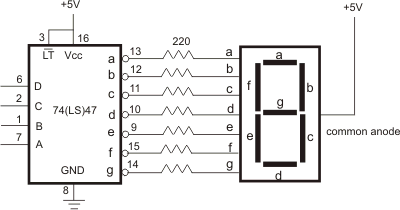
\includegraphics[scale=1.0]{images/DisplayResistors.png}
    \caption{Resistencias limitadoras de corriente}
    \label{Fig:Currentlimitingresistors}
\end{figure}

\pagebreak

\section{Resultados esperados}
\subsection{Funcionamiento completo}
Se requiere que al interconectar todos los circuitos el usuario interactúe con la entrada del \emph{dip-switch} y así seleccione el índice del dígito del año, mientras
este número se muestra directamente en el display de 7 segmentos.

\subsection{Optimización de recursos}
Recuerde que a pesar de obtener funciones separadas para las salidas de los Mapas de Karnaugh, es posible reutilizar operaciones entre los circuitos de salida.
Por ejemplo, piense en el siguiente caso hipotético en el que las funciones de salida de los Mapas de K. quedaran así:
$$ x = \bar A B \bar C + \bar A \bar C + \bar A$$
$$ y = AB\bar C + \bar C + B $$
$$ z = AB + \bar A \bar C + \bar A $$
$$ w = ABC + A\bar B \bar C + B $$

En la función $x$ aparecen varias veces $\bar A$ y $\bar C$, por lo que solamente es necesario utilizar una compuerta lógica para negar cada variable de entrada. Asimismo,
la variable negada $\bar A$ de la función $x$ puede reutilizarse en el circuito de la función $z$, donde aparece de nuevo. Incluso, el mintérmino completo de $x$ $(\bar A \bar C)$
se repite también en $z$, por lo que se posible reutilizar la salida de esa operación completa de $x$ directamente en $z$. 


\section{Conclusiones}
El funcionamiento del selector de índice es muy utilizado en electrónica digital y sirve para trasladar o codificar información única
en base a un índice o número que indica qué operación realizar. Esta operación es parte fundamental del funcionamiento de un microprocesador,
incluso de la tecnología actual.

\vspace{14pt}

En realidad, lo que se acaba de construir es conocido como un \textbf{Multiplexor} (coloquialmente MUX).
%ingreso de la bibliografía
%\bibliographystyle{apacite}
%\bibliography{biblio.bib}

\end{document} 


